
\documentclass[11pt,a4paper,openany]{report}
\usepackage[T1]{fontenc}
\usepackage[utf8]{inputenc}
\usepackage{lmodern}
\usepackage{microtype}
\usepackage{amsmath,amssymb,amsthm,mathtools,bm}
\usepackage{booktabs,array,longtable,tabularx}
\usepackage{xcolor}
\usepackage[margin=22mm,headheight=23pt]{geometry}
\usepackage{enumitem}
\usepackage{fancyhdr}
\usepackage{fancyvrb}
\usepackage{graphicx}
\usepackage{url}
\usepackage{xurl}
\usepackage{hyperref}
\definecolor{finblue}{HTML}{1F5A99}
\definecolor{fingreen}{HTML}{19733A}
\definecolor{finorange}{HTML}{D55E00}
\definecolor{finred}{HTML}{A61B1B}
\definecolor{finviolet}{HTML}{6A3D9A}
\definecolor{fingray}{HTML}{4D4D4D}

\hypersetup{
  unicode=true,
  colorlinks=true,
  linkcolor=finblue,
  citecolor=fingreen,
  urlcolor=finblue,
  pdftitle={FIN Research Programs P379--P393},
  pdfauthor={Krzysztof Żuchowski},
  pdfsubject={Proof-reflected certificates, global radial injectivity, noisy dynamics, and a first explicit operational realization},
  pdfkeywords={FIN, Lean, exact certificate, Bernstein polynomial, Lindemann-Weierstrass, radial injectivity, graph isometry, quantum comb, importance sampling, operational realization, dilation semigroup}
}
\pagestyle{fancy}
\fancyhf{}
\fancyhead[L]{\small FIN Programs P379--P393}
\fancyhead[R]{\small Release 10.33}
\fancyfoot[C]{\thepage}

\setlength{\parindent}{0pt}
\setlength{\parskip}{0.55em}
\setlist{nosep,leftmargin=2em}
\setcounter{tocdepth}{2}
\setcounter{secnumdepth}{3}
\emergencystretch=3em
\newcommand{\one}{\bm 1}
\newcommand{\C}{\mathbb C}
\newcommand{\R}{\mathbb R}
\newcommand{\Z}{\mathbb Z}
\newcommand{\statusProven}{\textcolor{fingreen}{[Proven]}}
\newcommand{\statusStrong}{\textcolor{finblue}{[Strong evidence]}}
\newcommand{\statusModerate}{\textcolor{finviolet}{[Moderate evidence]}}
\newcommand{\statusWeak}{\textcolor{fingray}{[Weak evidence]}}
\newcommand{\statusSpeculative}{\textcolor{finorange}{[Speculative]}}
\newcommand{\statusRefuted}{\textcolor{finred}{[Refuted]}}

\begin{document}
\hypersetup{pageanchor=false}
\begin{titlepage}
\centering
\vspace*{7mm}
{\Large\bfseries FIN --- Release 10.33\par}
\vspace{9mm}
{\Huge\bfseries Research Programs P379--P393\par}
\vspace{6mm}
{\Large Proof-reflected certificates, global radial injectivity,\\
noisy dynamics, and a first explicit operational realization\par}
\vspace{13mm}
{\Large Krzysztof \.Zuchowski\par}
\vspace{2mm}
{\normalsize Independent Researcher --- Fractal Information Theory Project\par}
\vspace{2mm}
{\normalsize ORCID:
\href{https://orcid.org/0009-0002-0909-3613}{0009-0002-0909-3613}\par}
\vspace{7mm}
{\large 31 July 2026\par}
{\normalsize Publication --- Preprint; Version 1.0.0\par}
\vfill
\begin{minipage}{0.92\textwidth}
\small
\textbf{Near-contact oscillatory certificate.}
\[
0.7073534379053974
\leq\mathcal N_{\rm osc}
\leq0.7073534683998260,
\qquad
\operatorname{width}<3.05\times10^{-8}.
\]

\textbf{Global strict radial theorem.}
\[
d\neq e,\quad d,e\in\mathbb N_0
\quad\Longrightarrow\quad
K_{\rm strict}(d)\neq K_{\rm strict}(e).
\]

Thirty-five exact terminal predicates are checked by Lean 4.28. One
positive-probability mathematical realization is constructed for the signed
resource. No selector, dimensional standard, calibrated laboratory
realization, role transfer, Standard Model, gravity, or Theory-of-Everything
closure is claimed.

\medskip
\textbf{Repository.}
\url{https://github.com/hyconiek/Fractal-Nadsoliton-Theory}

\textbf{License.} CC BY 4.0.
\end{minipage}
\vfill
\end{titlepage}
\hypersetup{pageanchor=true}
\pagenumbering{roman}
\chapter*{Publication statement}
\addcontentsline{toc}{chapter}{Publication statement}
This monograph reports every executed Program P379--P393 and recommends
Programs P394--P410. Exact proof, proof-kernel reflection, bounded numerical
evidence, conditional operational construction, and absent external evidence
are kept distinct. The legacy/strict split and all current strict-core
guardrails remain binding.

\tableofcontents
\clearpage
\pagenumbering{arabic}

\chapter*{Confidence convention}
\addcontentsline{toc}{chapter}{Confidence convention}

\begin{center}
\begingroup\small
\setlength{\tabcolsep}{2.5pt}
\renewcommand{\arraystretch}{1.16}
\begin{longtable}{@{}p{0.420\textwidth}p{0.420\textwidth}@{}}
\toprule
\textbf{Label} & \textbf{Meaning} \\
\midrule
\endhead
\textbf{\statusProven{}} & Mathematical proof, exact rational computation, proof-kernel-checked terminal predicate, or exhaustive finite result \\
\textbf{\statusStrong{}} & Reproducible high-precision or bounded finite computation with explicit limitations \\
\textbf{\statusModerate{}} & Model-dependent synthetic or local result \\
\textbf{[Conditional]} & Requires named preparations, encodings, standards, calibrations, or axioms \\
\textbf{\statusRefuted{}} & The declared proposition fails in its stated class \\
\textbf{[Blocked by external evidence]} & Independent data, hardware, calibration, custody, standards, or unblinding is required \\
\bottomrule
\end{longtable}
\endgroup
\end{center}

\chapter{Scientific scope and guardrails}

\section{The kernel split remains binding}

The legacy intermediate kernel is

\[
K_{\mathrm{legacy,ont}}(d)
=
4\ln2\,
\frac{\cos(\pi d/4+\pi/6)}{1+0.01d},
\]

whereas the strict working kernel is

\[
K_{\mathrm{strict,gate}}(d)
=
\frac{\cos((743/4000)d+13/80)}
{1+d^{9/5}}.
\]

P382 completes only the attenuation denominator after amplitude and phase have been separated. It is not an identity between the two full kernels.

\section{Ontology}

The repository order remains

\[
\text{nadsoliton}
\longrightarrow
\text{light}
\longrightarrow
\text{matter}
\longrightarrow
\text{emergent observer}.
\]

The nadsoliton is the primordial information in a solitonic state. No proof in this report assumes another informational substrate below it.

\section{Preserved open boundaries}

The following remain open:

\begin{itemize}
\item 
QW-2191 and a non-premise selector;

\item 
a source-independent complete legacy-to-strict map;

\item 
transfer of legacy electroweak or hierarchy roles;

\item 
internal length, time, action, mass, or energy standards;

\item 
calibrated laboratory preparation and measurement;

\item 
a unit-bearing nonproxy total action;

\item 
Standard Model or gravity generation;

\item 
Theory-of-Everything closure.

\end{itemize}

\chapter{Executive result table}

\begin{center}
\begingroup\small
\setlength{\tabcolsep}{2.5pt}
\renewcommand{\arraystretch}{1.16}
\begin{longtable}{@{}p{0.137\textwidth}p{0.417\textwidth}p{0.306\textwidth}@{}}
\toprule
\textbf{Program} & \textbf{Result} & \textbf{Status} \\
\midrule
\endhead
P379 & 35 exact terminal predicates checked by Lean & \statusProven{} /\allowbreak{} end-to-end reflection open \\
P380 & Oscillatory gap reduced to \(3.05\times10^{-8}\) & \statusProven{} \\
P381 & Strict kernel globally injective on \(\mathbb N_0\) & \statusProven{} \\
P382 & One damping naturality square; full completion fails & \statusProven{} /\allowbreak{} \statusRefuted{} \\
P383 & Exact \((2\pi\mathbb Z)^{66}\) coordinate gauge & \statusProven{} /\allowbreak{} global aliases open \\
P384 & No calibrated photonic pilot admitted & [Blocked] \\
P385 & Noisy adaptive upper and parallel lower bounds & \statusProven{} /\allowbreak{} optimum open \\
P386 & Clock-tube discrimination envelope & \statusProven{} /\allowbreak{} [Conditional] \\
P387 & Jordan Sampling Realization functor & \statusProven{} /\allowbreak{} physical execution conditional \\
P388 & Twenty forced cross-conversions refuted & \statusProven{} \\
P389 & Dilation semigroup does not select \(\rho\) & \statusProven{} \\
P390 & No independent QW hold-out admitted & [Blocked] \\
P391 & No dimensional standards bundle admitted & [Blocked] \\
P392 & No reservoir tomography bundle admitted & [Blocked] \\
P393 & No electroweak blind-test bundle admitted & [Blocked] \\
\bottomrule
\end{longtable}
\endgroup
\end{center}

\chapter{P379 --- what proof-kernel reflection now means}

\section{Reflected predicates}

The generated Lean source contains:

\begin{center}
\begingroup\small
\setlength{\tabcolsep}{2.5pt}
\renewcommand{\arraystretch}{1.16}
\begin{longtable}{@{}p{0.420\textwidth}p{0.420\textwidth}@{}}
\toprule
\textbf{Predicate class} & \textbf{Count} \\
\midrule
\endhead
Krawczyk lower/\allowbreak{}upper containment & 24 \\
Certified weight signs & 7 \\
Bernstein lower/\allowbreak{}upper bounds & 2 \\
Weak-duality order and contact gap & 2 \\
\textbf{Total} & \textbf{35} \\
\bottomrule
\end{longtable}
\endgroup
\end{center}

Each rational comparison

\[
\frac ab<\frac cd
\]

is converted to an integer proposition

\[
ad<cb
\]

with positive denominators. Lean evaluates the exact integer proposition by kernel-checked decision.

\section{What is no longer trusted}

A silent floating comparison is not trusted. Decimal display values are not the proof objects. Hash identity alone is not the proof object. The terminal containment, sign, feasibility, order, and gap statements are represented by exact integers.

\section{What is still trusted}

The following generators remain Python implementations:

\begin{itemize}
\item 
Taylor/\allowbreak{}Lagrange cosine intervals;

\item 
fifth-root brackets;

\item 
interval matrix arithmetic;

\item 
Krawczyk construction;

\item 
Bernstein subdivision;

\item 
conversion from archived mathematical inputs to terminal rational claims.

\end{itemize}

Therefore P379 is a genuine reduction of the trusted base, not a complete formalization of the numerical proof pipeline.

\begin{figure}[htbp]
\centering
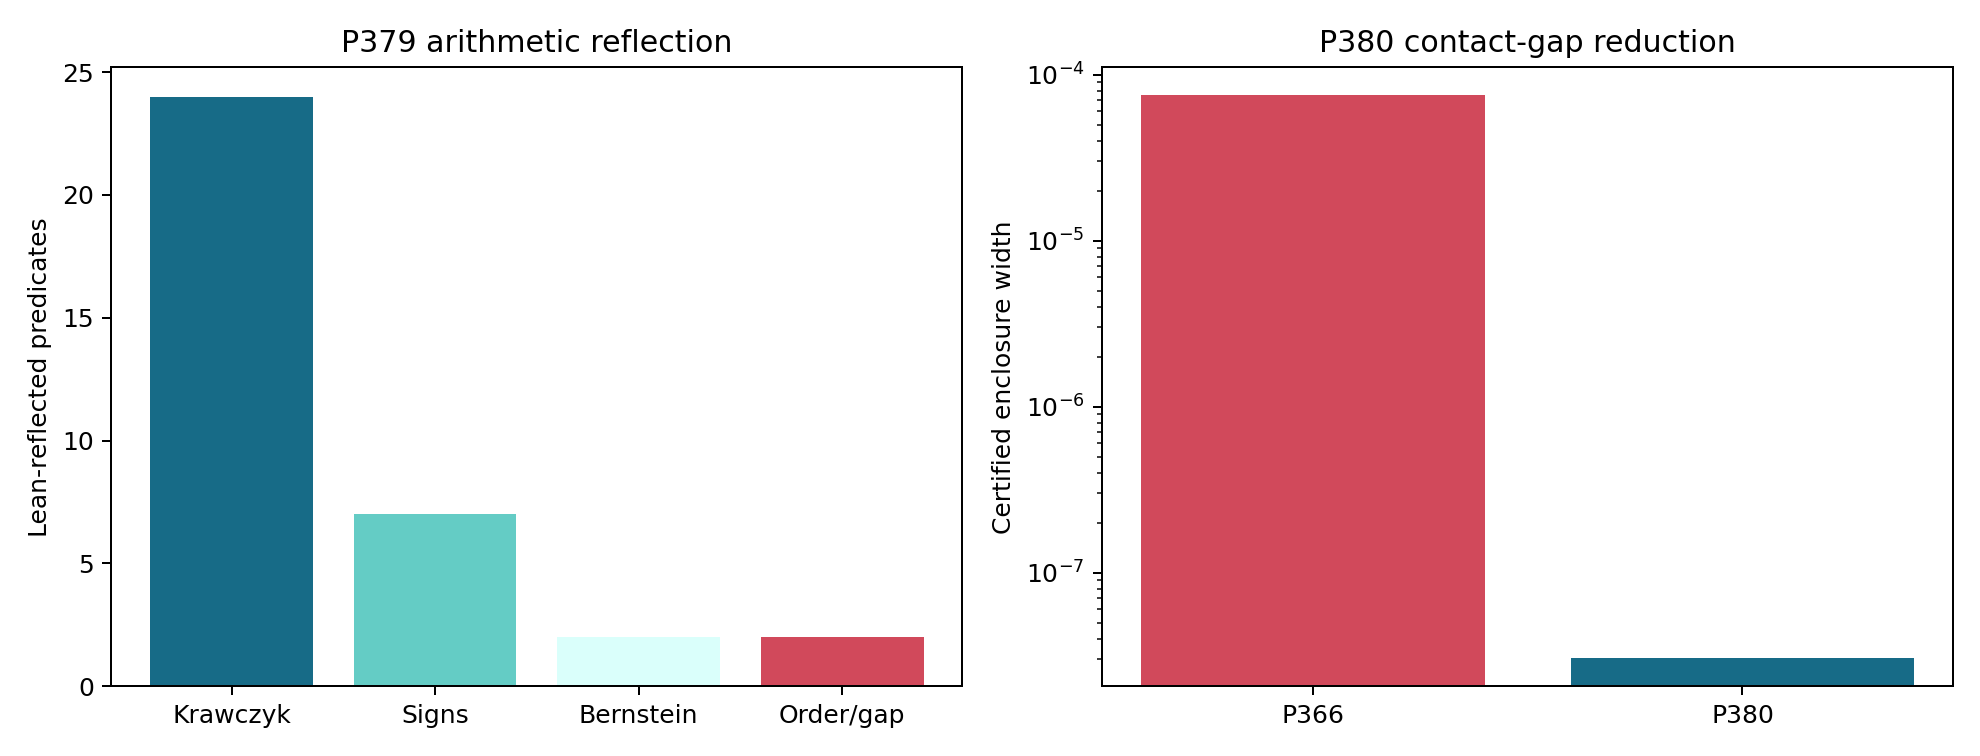
\includegraphics[width=0.97\textwidth]{FIN_Programs_379_393_Figures/p379_p380_reflection_contact.png}
\caption{Lean-reflected terminal predicates and the reduction of the exact oscillatory primal-dual gap.}
\end{figure}

\chapter{P380 --- near-contact oscillatory extremality}

\section{Why the old basis was inefficient}

The raw degree-eleven monomial representation contains coefficients of very different magnitudes. Feasibility is a statement about a bounded function, but monomial coefficients are a poorly conditioned coordinate system for that statement.

P380 optimizes and freezes the polynomial in the Bernstein basis. Local Bernstein coefficients on dyadic cells directly bound the polynomial.

\section{Exact normalization}

Let \(b_0,\ldots,b_{11}\in\mathbb Q\) be the frozen Bernstein coefficients. On all \(2^{14}\) dyadic cells, exact de Casteljau subdivision gives rational extrema \(L,U\). Define

\[
p_{\mathrm{safe}}(x)
=
\frac{p_{\mathrm{raw}}(x)-U}{U-L}.
\]

Every local Bernstein coefficient then belongs to \([-1,0]\). Therefore

\[
-1\leq p_{\mathrm{safe}}(x)\leq0
\qquad(0\leq x\leq1).
\]

\section{Primal-dual result}

The exact dual lower endpoint is

\[
0.7073534379053974.
\]

The existing exact seven-atom Krawczyk primal gives

\[
0.7073534683998260.
\]

Weak duality proves the global enclosure stated in the abstract.

\section{Interpretation}

The result establishes a nearly closed extremal problem in classical signed Hausdorff moment theory. It does not choose a physical ontology for signed mass. P387 supplies one positive-probability operational encoding, but it is not forced uniquely.

\chapter{P381 --- the global strict-distance theorem}

\section{Statement}

For

\[
k(d)=
\frac{\cos(x_d)}{1+d^{9/5}},
\qquad
x_d=\frac{743d+650}{4000},
\]

the restriction

\[
k:\mathbb N_0\longrightarrow\mathbb R
\]

is injective.

\section{Proof}

For every \(d\in\mathbb N_0\), \(x_d\) is a positive rational and

\[
a_d=\frac{1}{1+d^{9/5}}
\]

is a nonzero algebraic number.

Assume \(d\neq e\) and \(k(d)=k(e)\). Then

\[
a_d(e^{ix_d}+e^{-ix_d})
-
a_e(e^{ix_e}+e^{-ix_e})
=0.
\]

The four exponents

\[
ix_d,\quad -ix_d,\quad ix_e,\quad -ix_e
\]

are distinct algebraic numbers. The Lindemann--Weierstrass theorem says that their exponentials are linearly independent over the algebraic numbers. The displayed nontrivial relation is impossible.

Therefore \(k(d)\neq k(e)\).

\section{Categorical consequence}

P368 identified the maximal radial naturality category as maps preserving distance modulo equality of kernel values. P381 removes the quotient ambiguity globally:

\[
k(d_H(fx,fy))=k(d_G(x,y))
\quad\Longleftrightarrow\quad
d_H(fx,fy)=d_G(x,y).
\]

This conclusion holds on integer shortest-path metrics of arbitrary finite diameter.

\section{Boundary}

The theorem is formula-specific. It does not say that the same function is natural on continuous metric spaces, nor that the legacy kernel shares its category, nor that physical spacetime is a graph metric.

\chapter{P382 --- one bridge atom, and no more}

\section{The exact square}

Define

\[
a_L(d)=\frac{1}{1+0.01d},
\qquad
a_S(d)=\frac{1}{1+d^{9/5}}.
\]

Then

\[
C_{\mathrm{damp}}(d)a_L(d)=a_S(d)
\]

identically.

For an isometric embedding \(f:G\to H\),

\[
C_{\mathrm{damp}}(d_H(fx,fy))
=
C_{\mathrm{damp}}(d_G(x,y)).
\]

Thus pullback commutes with entrywise damping completion.

\section{Why this is not a source theorem}

The formula for \(C_{\mathrm{damp}}\) already contains:

\begin{itemize}
\item 
the strict unit coefficient;

\item 
the strict exponent \(9/5\);

\item 
the legacy coefficient \(0.01\).

\end{itemize}

It packages a target comparison. It does not derive strict compression from legacy data.

\section{Full-kernel falsification}

After amplitude absorption and damping replacement, the legacy phase remains

\[
\cos(\pi d/4+\pi/6),
\]

not

\[
\cos((743/4000)d+13/80).
\]

The \(C_{12}\) relative profile residual is approximately \(0.9944\). Damping alone therefore fails as a full completion.

\chapter{P383--P384 --- photonic gauge and physical boundary}

\section{Exact coordinate gauge}

Each component phase appears only through \(e^{\pm i\varphi_j}\). Hence

\[
\varphi_j\sim\varphi_j+2\pi n_j,
\qquad
n_j\in\mathbb Z.
\]

The natural canonical chart is

\[
\mathbb R_+^{66}\times(-\pi,\pi]^{66}.
\]

\section{Finite audit}

For all 66 components:

\begin{itemize}
\item 
a single \(2\pi\) shift has maximum transfer defect below \(8.0\times10^{-16}\);

\item 
32 random combined phase-lattice shifts have maximum defect below \(3.8\times10^{-15}\);

\item 
every tested single \(\pi\) shift has defect at least \(0.285\);

\item 
every tested \(0.01\) component-loss shift has defect at least \(4.99\times10^{-3}\).

\end{itemize}

These numbers identify coordinate gauges, not every possible distant compensating alias.

\begin{figure}[htbp]
\centering
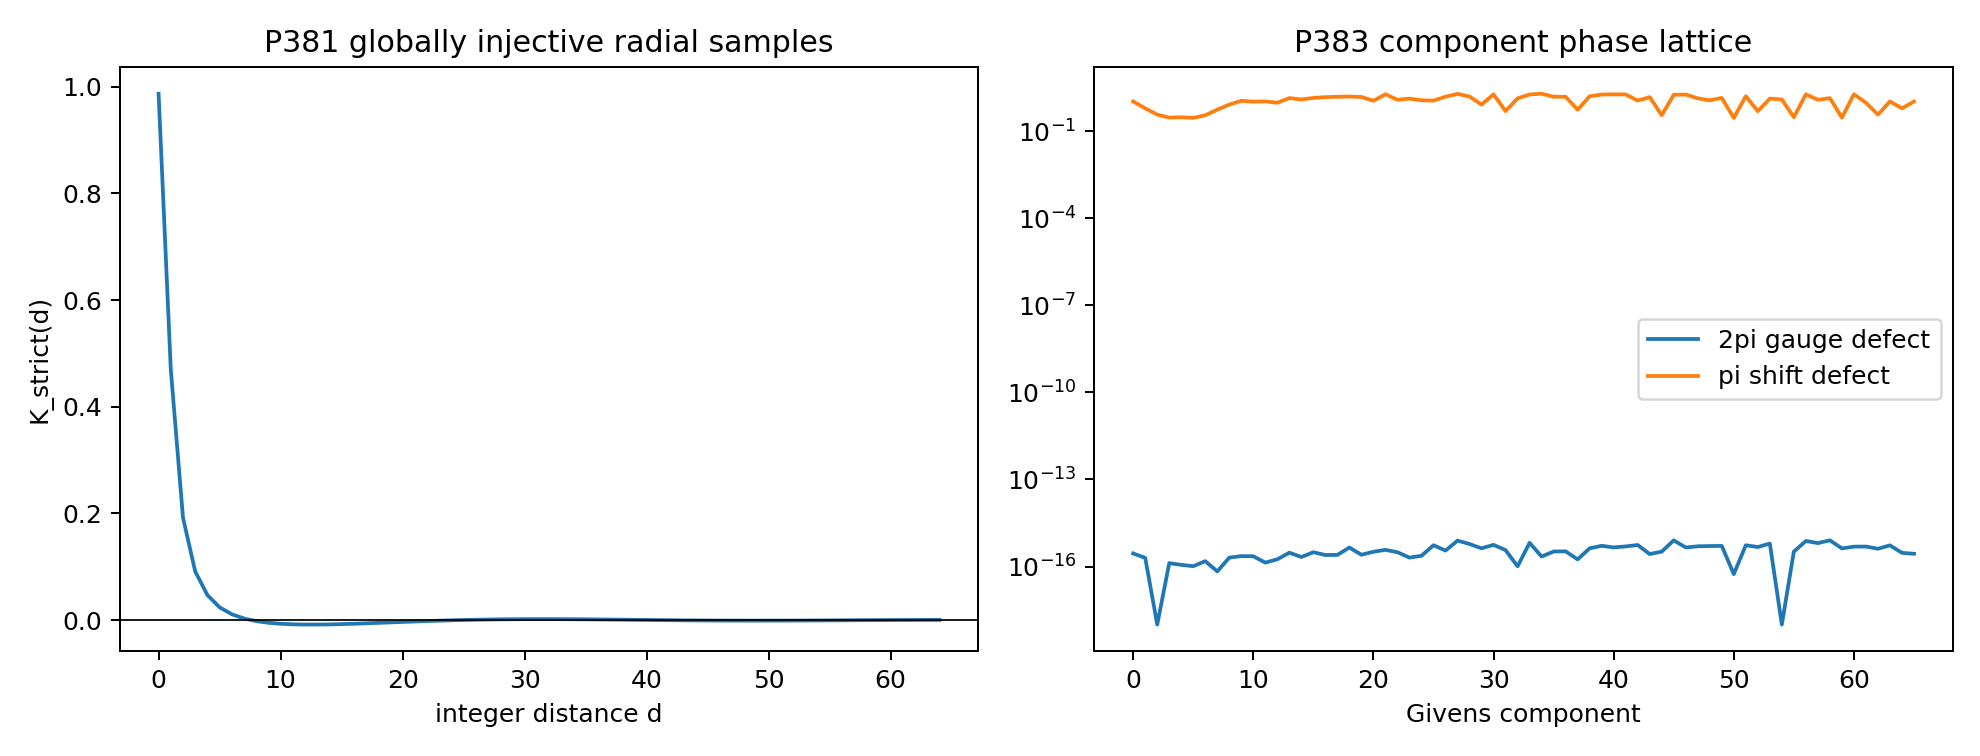
\includegraphics[width=0.97\textwidth]{FIN_Programs_379_393_Figures/p381_p383_injectivity_gauge.png}
\caption{Global strict radial injectivity diagnostics and the photonic component-phase coordinate gauge.}
\end{figure}

\section{External boundary}

P384 finds no admitted calibrated pilot. A physical pilot must supply complex transfer calibration, detector response, timestamps, preparation records, independent custody, a frozen protocol, and an unmodified hold-out report.

\chapter{P385 --- the noisy-comb sandwich}

\section{Declared reduced channel}

Restrict to the two extremal eigenmodes of the relative generator. Let:

\begin{itemize}
\item 
\(\eta\in[0,1]\) be independent heralded survival per call;

\item 
\(q\in[0,1]\) be eigenbasis coherence retention;

\item 
\(\theta=t\Delta/2\).

\end{itemize}

The two one-use states have off-diagonal phases \(e^{\pm i\theta}\), attenuated by \(q\). Orthogonal erasure flags contribute only on surviving branches.

\section{One-use distance}

The exact one-use half-distance is

\[
\delta_1=\eta q|\sin\theta|.
\]

\section{Adaptive upper bound}

The hybrid/\allowbreak{}telescoping argument replaces oracle calls one at a time. Trace-distance contractivity under common adaptive controls gives

\[
D_n^{\mathrm{adaptive}}
\leq
\min(1,n\delta_1).
\]

\section{Feasible lower bounds}

For independent probes, condition on \(k\) surviving calls:

\[
L_{\mathrm{prod}}
=
\sum_{k=1}^n
\binom nk\eta^k(1-\eta)^{n-k}
\frac12
\left\|
\rho_+^{\otimes k}
-
\rho_-^{\otimes k}
\right\|_1.
\]

For the GHZ strategy, only the all-surviving coherent branch is used:

\[
L_{\mathrm{GHZ}}
=
\eta^nq^n|\sin(n\theta)|.
\]

Therefore

\[
\max(L_{\mathrm{prod}},L_{\mathrm{GHZ}})
\leq
D_n^{\mathrm{adaptive}}
\leq
\min(1,n\eta q|\sin\theta|).
\]

In the ideal case \(\eta=q=1\), the GHZ lower recovers the P371 first-branch optimum.

\section{Open problem}

The largest gap in the declared audit is approximately \(0.5591\). Closing it requires either:

\begin{itemize}
\item 
a channel-comb SDP with a dual certificate;

\item 
an erasure-tolerant entangled code;

\item 
a sharper adaptive contraction theorem;

\item 
a proof that one of the displayed strategies is optimal in a restricted noise class.

\end{itemize}

\chapter{P386 --- clocks deform predictions into tubes}

If the true dimensionless time lies in

\[
\tau\in[\widehat\tau-\epsilon,\widehat\tau+\epsilon]
\]

and the interval remains on the first P371 branch, monotonicity gives

\[
\sin\!\left(
\frac{n\Delta(\widehat\tau-\epsilon)}2
\right)
\leq
D_n(\tau)
\leq
\sin\!\left(
\frac{n\Delta(\widehat\tau+\epsilon)}2
\right).
\]

Endpoints are clipped to the physical branch \([0,\pi/(n\Delta)]\).

\begin{figure}[htbp]
\centering
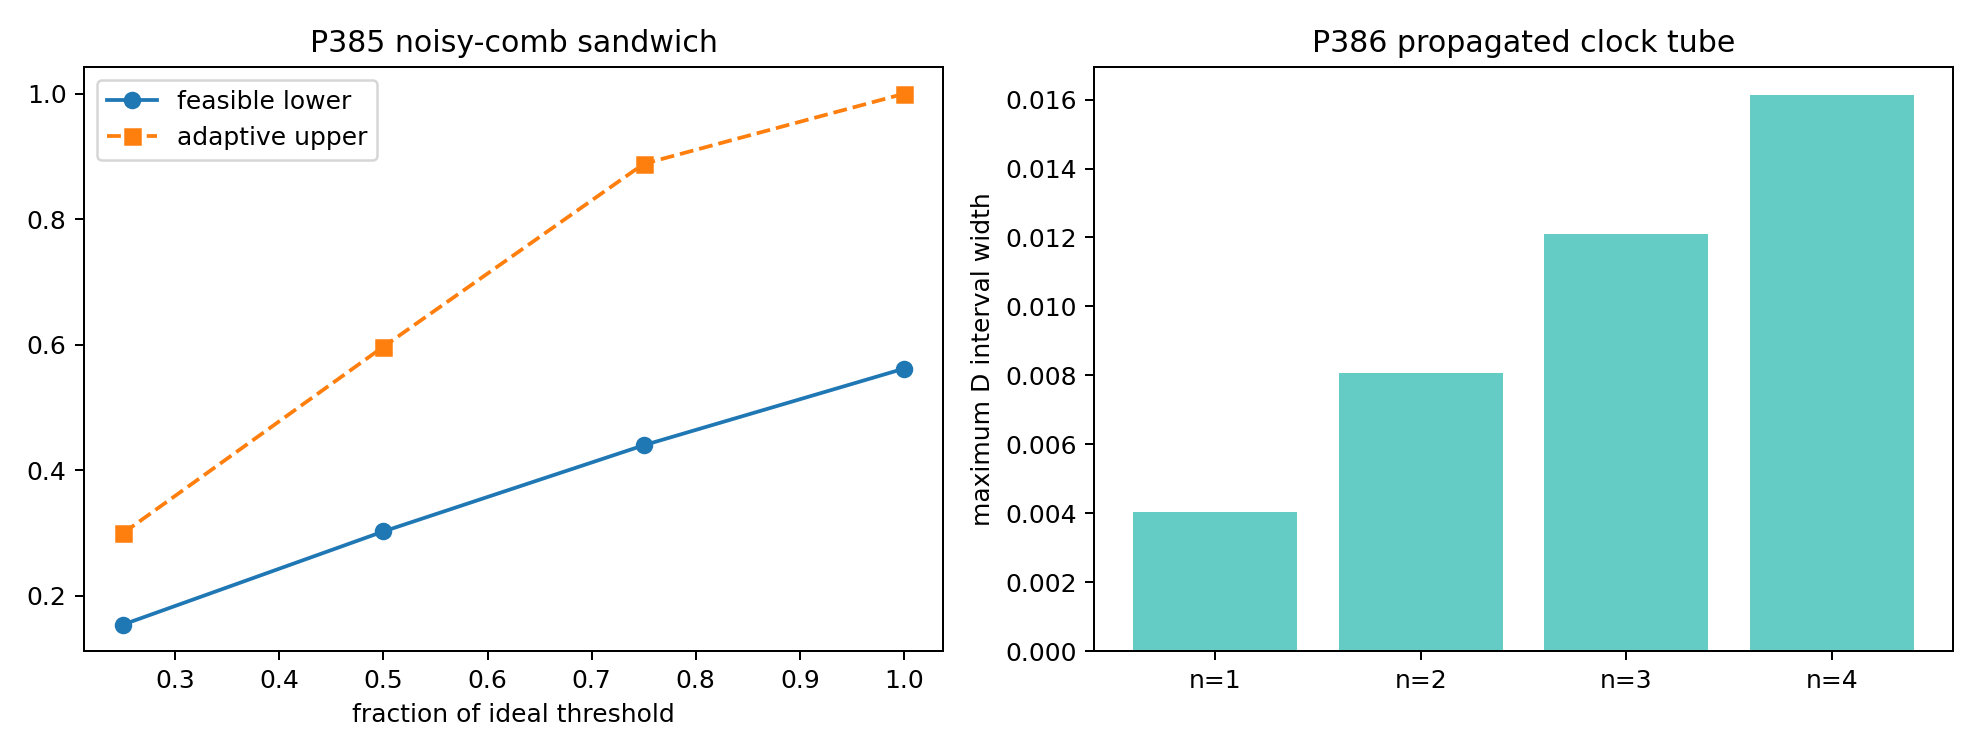
\includegraphics[width=0.97\textwidth]{FIN_Programs_379_393_Figures/p385_p386_loss_clock.png}
\caption{The declared noisy-comb lower/upper sandwich and propagated clock-calibration tubes.}
\end{figure}

The result separates two questions:

\begin{enumerate}
\item 
what FIN predicts after a clock map is supplied;

\item 
how the clock map is calibrated experimentally.

\end{enumerate}

Only the first is solved here.

\chapter{P387 --- Jordan Sampling Realization}

\section{Category of source objects}

The source objects are finite signed measures

\[
\mu=\sum_iw_i\delta_{x_i}.
\]

Positive column-stochastic maps act on the signed weight vector.

\section{Operational preparation}

Define

\[
V=\sum_i|w_i|,
\qquad
q_i=\frac{|w_i|}{V},
\qquad
s_i=\operatorname{sgn}(w_i).
\]

The preparation distribution \(q\) is ordinary and positive.

\section{Instrument and record}

One trial produces

\[
(i,x_i,s_i,\mathrm{run\ id},\mathrm{timestamp}).
\]

For mathematical reconstruction, the minimal record is \((i,x_i,s_i)\). Laboratory timestamps and run identifiers are required for custody and drift tests.

\section{Estimator identity}

For any function \(f\),

\[
\widehat f=Vs_if(x_i)
\]

is unbiased:

\[
\mathbb E_q[\widehat f]
=
\sum_iw_if(x_i).
\]

In particular, \(f(x)=x^k\) reconstructs the signed moments.

\section{Resource monotonicity}

The Jordan negative mass is

\[
\mathcal N(\mu)
=
\frac{\|\mu\|_{\mathrm{TV}}-\mu(X)}2.
\]

For a positive mass-preserving Markov map \(T\),

\[
\|T\mu\|_{\mathrm{TV}}
\leq
\|\mu\|_{\mathrm{TV}},
\qquad
(T\mu)(X)=\mu(X).
\]

Therefore

\[
\mathcal N(T\mu)\leq\mathcal N(\mu).
\]

\section{What has and has not been constructed}

Constructed mathematically:

\begin{itemize}
\item 
state/\allowbreak{}preparation;

\item 
free dynamics;

\item 
instrument;

\item 
score;

\item 
record schema;

\item 
monotone;

\item 
reconstruction theorem.

\end{itemize}

Not constructed physically:

\begin{itemize}
\item 
a device realizing the nodes and probabilities;

\item 
a dimensional clock;

\item 
detector calibration;

\item 
environmental model;

\item 
independent raw-event custody;

\item 
a theorem that nature uses this realization.

\end{itemize}

\begin{figure}[htbp]
\centering
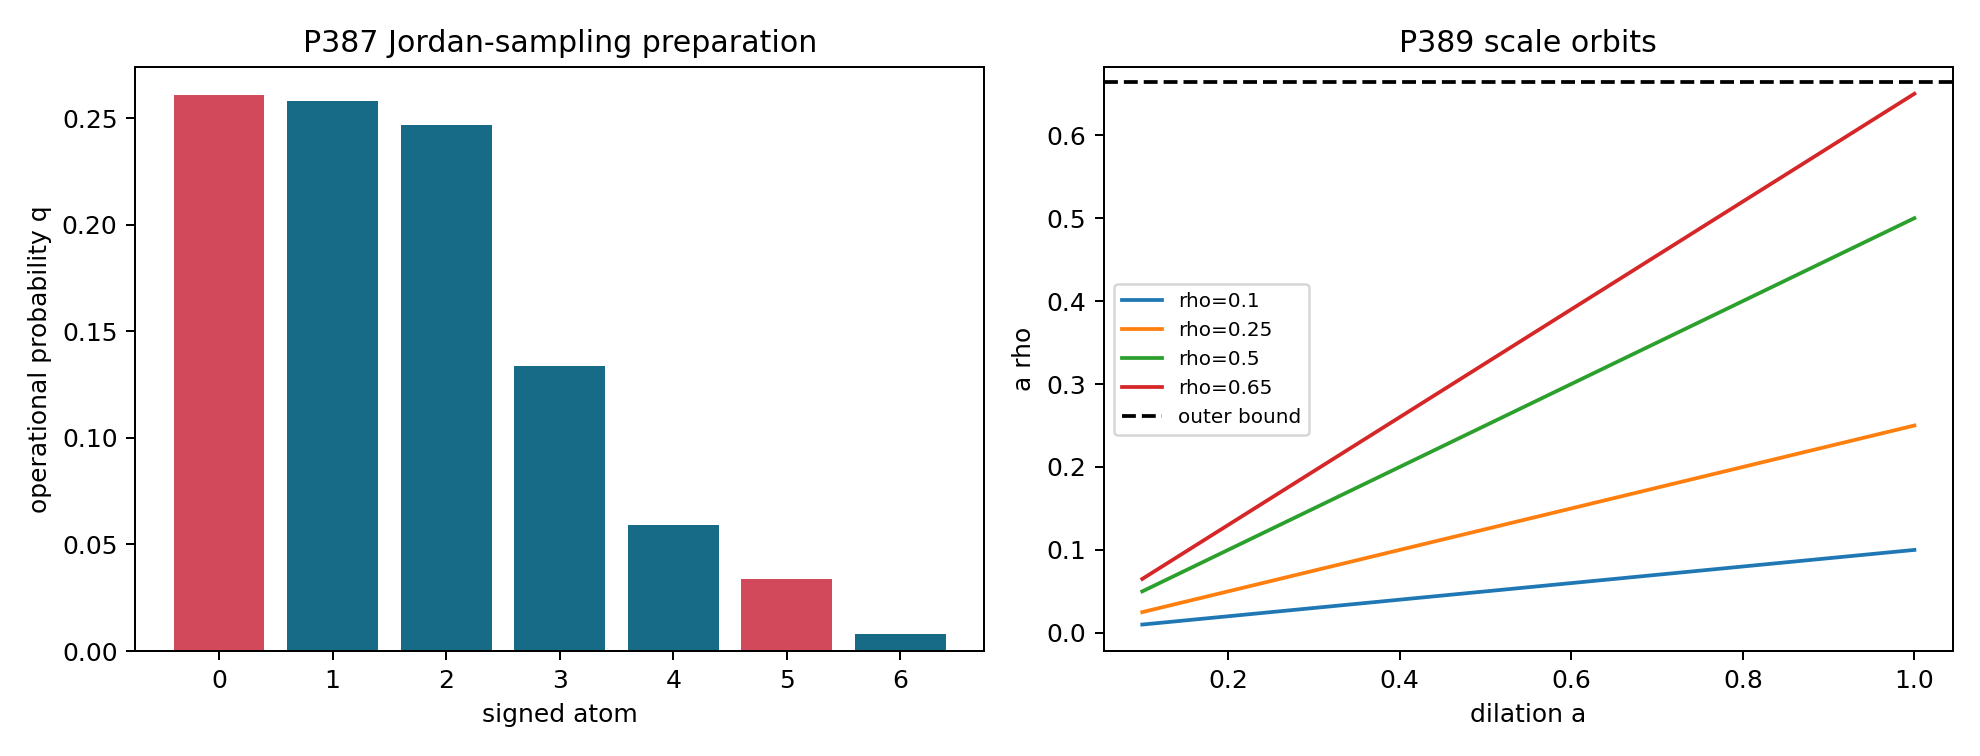
\includegraphics[width=0.97\textwidth]{FIN_Programs_379_393_Figures/p387_p389_realization_scale.png}
\caption{Positive Jordan-sampling preparation probabilities and the noncanonical outer-scale dilation orbits.}
\end{figure}

\chapter{P388 --- conversion is not implied by co-listing resources}

Let

\[
\mathbf r=(r_1,\ldots,r_5)\in\mathbb N^5.
\]

For every ordered pair \(i\neq j\), the generator

\[
e_i=(0,\ldots,1,\ldots,0)
\]

has \(r_i>0\) and \(r_j=0\). Hence the minimal signature cannot prove

\[
r_i>0\Longrightarrow r_j>0.
\]

All twenty directed cross-implications fail.

Identity conversions exist. Reset maps destroy resources. Catalysts cannot create new comparisons because

\[
\mathbf a+\mathbf c\geq\mathbf b+\mathbf c
\quad\Longrightarrow\quad
\mathbf a\geq\mathbf b.
\]

This is not a universal physical no-go. A concrete coupling functor can add conversions, but the coupling must be an additional theorem or axiom.

\chapter{P389 --- why the analytic extension has no preferred scale}

For

\[
F_\rho(z)=\sum_{d\geq0}K(d)\rho^dz^d,
\]

define

\[
(D_aF)(z)=F(az).
\]

Then

\[
D_aF_\rho=F_{a\rho},
\qquad
D_aD_b=D_{ab}.
\]

The coordinate

\[
t=-\log\rho
\]

converts multiplication into addition. However, an invariant positive selector would have to satisfy

\[
\rho=a\rho
\]

for every admissible \(a\), including \(a=1/2\). This forces \(\rho=0\), which is outside the positive family.

Therefore the semigroup provides evolution or coarse-graining order, but not a preferred origin, unit, or interior scale.

\chapter{P390--P393 --- external gates}

\begin{center}
\begingroup\small
\setlength{\tabcolsep}{2.5pt}
\renewcommand{\arraystretch}{1.16}
\begin{longtable}{@{}p{0.195\textwidth}p{0.420\textwidth}p{0.245\textwidth}@{}}
\toprule
\textbf{Program} & \textbf{Required external object} & \textbf{Current status} \\
\midrule
\endhead
P390 & Independent QW hold-out, frozen before evaluation & Not admitted \\
P391 & Traceable \((\ell_*,\tau_*,\hbar_*)\) standards package & Not admitted \\
P392 & Physical reservoir process-tomography record & Not admitted \\
P393 & Blinded electroweak conditional-test bundle & Not admitted \\
\bottomrule
\end{longtable}
\endgroup
\end{center}

Every bundle must include:

\begin{itemize}
\item 
distinct provider, registrar, and analyst;

\item 
raw-record hash;

\item 
calibration hash;

\item 
freeze timestamp;

\item 
unblinding authorization;

\item 
an immutable failure report.

\end{itemize}

\chapter{Newly constructed theoretical objects}

\begin{center}
\begingroup\small
\setlength{\tabcolsep}{2.5pt}
\renewcommand{\arraystretch}{1.16}
\begin{longtable}{@{}p{0.247\textwidth}p{0.207\textwidth}p{0.214\textwidth}p{0.192\textwidth}@{}}
\toprule
\textbf{Object} & \textbf{Definition} & \textbf{What it resolves} & \textbf{What remains open} \\
\midrule
\endhead
O121 Kernel-Reflected Terminal Certificate & 35 exact Lean-decided integer predicates & Terminal arithmetic trust & End-to-end algorithm reflection \\
O122 Near-Contact Bernstein Extremal Pair & Exact dual plus P366 primal & Oscillatory gap below \(10^{-7}\) & Exact equality and uniqueness \\
O123 Global Strict Radial Embedding Theorem & Injectivity of \(K_{\mathrm{strict}}\) on \(\mathbb N_0\) & Global graph-distance naturality & Continuous metrics and other kernels \\
O124 Damping-Completion Natural Transformation & \(C_{\mathrm{damp}}\) entrywise radial multiplier & One bridge square & Source of \(9/5\), phase, amplitude \\
O125 Photonic Component Gauge Quotient Chart & \(\mathbb R_+^{66}\times\mathbb T^{66}\) & Coordinate periodicity & Global nonlocal aliases \\
O126 Heralded Noisy-Comb Sandwich & Parallel lower and adaptive hybrid upper & Quantified noisy discrimination & Exact optimum \\
O127 Clock-Tube Discrimination Envelope & Monotone image of a calibrated time interval & Robust prediction & Clock source \\
O128 Jordan Sampling Realization Functor & Positive sampling with signed importance score & One complete mathematical A5 instance & Laboratory realization \\
O129 Resource Conversion Obstruction Matrix & Twenty generator countermodels & No forced cross-generation & Model-specific couplings \\
O130 Outer-Scale Dilation Torsor & Multiplicative \(\rho\)-orbit & Semigroup canonicality no-go & New boundary/\allowbreak{}normalization law \\
\bottomrule
\end{longtable}
\endgroup
\end{center}

\chapter{Falsification ledger}

\begin{center}
\begingroup\small
\setlength{\tabcolsep}{2.5pt}
\renewcommand{\arraystretch}{1.16}
\begin{longtable}{@{}p{0.287\textwidth}p{0.379\textwidth}p{0.193\textwidth}@{}}
\toprule
\textbf{Candidate conclusion} & \textbf{Falsification attempt} & \textbf{Verdict} \\
\midrule
\endhead
P380 is only floating optimization & Rational freezing, exact dyadic subdivision, Krawczyk primal, Lean terminal predicates & Survives in declared scope \\
Strict distance values may collide at large \(d\) & Lindemann--Weierstrass contradiction & Refuted globally \\
Damping completes legacy into strict & Full-profile residual on \(C_{12}\) & Refuted \\
Every photonic phase shift is physical & Independent \(2\pi\) lattice shifts & Refuted; exact gauge \\
Coordinate audit proves global identifiability & Distant compensating aliases not classified & Not established \\
P371 survives noise unchanged & Loss/\allowbreak{}dephasing sandwich differs from ideal sine law & Refuted \\
Clock uncertainty is negligible & Explicit tube propagation & Quantified, not erased \\
Signed mass requires negative probability & JSR positive probability construction & Refuted \\
Five resources automatically generate each other & Twenty generator countermodels & Refuted in minimal category \\
Analytic semigroup selects one \(\rho\) & Dilation-invariant selector test & Refuted \\
Code can close external physics & Custody and calibration requirements & Refuted \\
\bottomrule
\end{longtable}
\endgroup
\end{center}

\chapter{Current scientific interpretation}

The strongest defensible interpretation after P379--P393 is:

\begin{quote}\itshape
FIN is a dimensionless spectral-operator and signed-resource framework with a globally faithful strict radial graph geometry, nearly closed exact signed-moment certificates, conditional noisy dynamics, and at least one explicit positive-probability operational realization. It still lacks a calibrated empirical realization and internal dimensional standards.

\end{quote}

The previous realization gap has split into two layers:

\[
\mathcal R_{\mathrm{math}}
:
\text{one FIN signed resource}
\longrightarrow
\text{preparation, free channels, instrument, score, record schema},
\]

which P387 constructs, and

\[
\mathcal R_{\mathrm{lab}}
:
\mathcal R_{\mathrm{math}}
\longrightarrow
\text{calibrated apparatus and independent raw records},
\]

which remains external.

No amount of exact spectral calculus can replace the empirical content of \(\mathcal R_{\mathrm{lab}}\).

\chapter{Recommended Programs P394--P410}

\section{P394 --- end-to-end proof-assistant reflection}

Formalize:

\begin{itemize}
\item 
rational interval arithmetic;

\item 
fifth-root bracketing;

\item 
Taylor/\allowbreak{}Lagrange cosine bounds;

\item 
de Casteljau subdivision;

\item 
Krawczyk inclusion;

\item 
weak duality.

\end{itemize}

Success means the proof assistant derives the terminal predicates rather than only checking their integer forms.

\section{P395 --- exact contact geometry and uniqueness}

Use the \(3.05\times10^{-8}\) gap to identify the exact active contact pattern. Attempt:

\begin{itemize}
\item 
interval isolation of all dual extrema;

\item 
complementary-slackness equations;

\item 
uniqueness of the signed extremizer;

\item 
an algebraic or transcendental obstruction to exact finite contact.

\end{itemize}

\section{P396 --- formal global injectivity}

Import or formalize the required Lindemann--Weierstrass corollary and prove P381 in a proof assistant. Separate:

\begin{itemize}
\item 
algebraicity of \(d^{9/5}\);

\item 
distinctness of the four exponents;

\item 
exponential linear independence;

\item 
categorical corollary.

\end{itemize}

\section{\texorpdfstring{P397 --- source audit for \(C_{\mathrm{damp}}\)}{P397 --- source audit for C\_damp}}

Do not repeat the generic bridge. Ask one question:

\begin{quote}\itshape
Can a declared monoid/\allowbreak{}RG/\allowbreak{}coarse-graining law generate \((1+0.01d)/(1+d^{9/5})\) without reading the strict target?

\end{quote}

Prove a source theorem or a finite no-go for the declared provider class.

\section{P398 --- global photonic quotient identifiability}

Classify all parameter pairs in the canonical chart that produce the same complex transfer matrix. Determine:

\begin{itemize}
\item 
the exact gauge group;

\item 
distant aliases;

\item 
singular strata;

\item 
the minimum multitime calibration design.

\end{itemize}

\section{P399 --- calibrated photonic pilot}

External program. Require complex transfer tomography, detector calibration, raw timestamps, a frozen protocol, custody separation, and one-shot evaluation.

\section{P400 --- exact noisy adaptive-comb optimum}

Formulate the heralded loss/\allowbreak{}dephasing process as a finite comb SDP. Produce:

\begin{itemize}
\item 
feasible primal strategy;

\item 
dual upper certificate;

\item 
quantified gap;

\item 
a theorem identifying any regime where GHZ or product probes are optimal.

\end{itemize}

\section{P401 --- full twelve-mode noisy dynamics}

Lift P385 from the extremal two-mode subspace to:

\begin{itemize}
\item 
all twelve modes;

\item 
component loss;

\item 
dephasing;

\item 
detector confusion;

\item 
clock uncertainty.

\end{itemize}

Distinguish a physical channel from postselected conditional statistics.

\section{P402 --- clock-robust design with a supplied anchor}

Optimize sample times against the complete P386 prediction tube. The objective should maximize worst-case discrimination after calibration, not merely minimize interpolation error.

\section{P403 --- executable Jordan-sampling experiment}

Turn O128 into an executable specification:

\begin{itemize}
\item 
preparation probabilities;

\item 
atom encoder;

\item 
sign register;

\item 
randomization audit;

\item 
event schema;

\item 
estimator;

\item 
preregistered confidence intervals;

\item 
raw-record validator.

\end{itemize}

This remains a hypothesis of laboratory realization until physically run.

\section{P404 --- natural transformations among operational semantics}

Use the five P373 operational categories, not only their grades. Classify typed functors that preserve preparations, channels, instruments, and monotones.

\section{P405 --- sign-to-phase or sign-to-asymmetry coupling}

Test whether the JSR sign record can couple naturally to:

\begin{itemize}
\item 
dephasing coherence;

\item 
reflection asymmetry;

\item 
the P2718 chiral marker.

\end{itemize}

Reject any construction that merely relabels the sign as a strict selector.

\section{P406 --- canonical scale with one new boundary law}

Add exactly one candidate:

\begin{itemize}
\item 
normalized semigroup generator;

\item 
RG boundary condition;

\item 
apparatus resolution;

\item 
entropy reference cell.

\end{itemize}

Determine whether it selects \(\rho\), and state explicitly whether the result is strict, conditional, or target-defined.

\section{P407--P410 --- external falsification}

\begin{itemize}
\item 
P407: independent QW hold-out;

\item 
P408: dimensional standards package;

\item 
P409: physical reservoir process tomography;

\item 
P410: electroweak blind test.

\end{itemize}

Repository code may validate manifests but may not manufacture evidential status.

\section{Recommended immediate order}

\[
\boxed{
\mathrm{P394}
\longrightarrow
\mathrm{P395}
\longrightarrow
\mathrm{P396}
\longrightarrow
\mathrm{P400}
\longrightarrow
\mathrm{P403}
}.
\]

\chapter{Final conclusion}

P379--P393 produces three theorem-level advances.

First, the oscillatory signed-resource problem is now nearly closed with a proof-kernel-checked terminal certificate gap below \(10^{-7}\).

Second, strict radial geometry is globally faithful on integer graph distances. The earlier quotient category is not merely finite-range evidence: it is the ordinary isometric category for every finite integer-distance carrier.

Third, one previously abstract bridge has been constructed explicitly. Jordan Sampling Realization converts the signed measure into positive preparation probabilities, free Markov dynamics, an instrument, a score, and a record schema. This establishes mathematical operational realizability without pretending that signed mass is negative probability.

The corresponding laboratory bridge remains absent. Dimensional standards, detector calibration, custody, and external records cannot be generated by the spectral theorem or by repository code.

The deepest surviving interpretation is therefore:

\begin{quote}\itshape
FIN has matured into a rigorous dimensionless spectral and operational resource framework with global strict graph geometry and one explicit operational realization. Its remaining transition to physics is an empirical-calibration problem plus the independent selector and dimensional source obstructions, not another identity inside the functional calculus.

\end{quote}

\chapter{Reproducibility}

Run:

\begin{itemize}
\item 
MPLCONFIGDIR=/\allowbreak{}tmp/\allowbreak{}mpl-fin-1033 python3 fin\_programs\_379\_393.py

\item 
MPLCONFIGDIR=/\allowbreak{}tmp/\allowbreak{}mpl-fin-1033 python3 -m unittest -v test\_fin\_programs\_379\_393.py

\end{itemize}

Expected result: 16 tests passed, zero failed. Both Lean 4.28 files must compile. P384 and P390--P393 remain external admission gates.

\chapter{Suggested citation}

\.Zuchowski, K. (2026). \emph{FIN Research Programs P379--P393: Proof-Reflected Certificates, Global Radial Injectivity, Noisy Dynamics, and a First Explicit Operational Realization} (Release 10.33; Version 1.0.0) [Preprint]. Zenodo.


\clearpage
\chapter*{Reproduction certificate}
\addcontentsline{toc}{chapter}{Reproduction certificate}
\begin{Verbatim}[fontsize=\small]
MPLCONFIGDIR=/tmp/mpl-fin-1033 \
python3 fin_programs_379_393.py

MPLCONFIGDIR=/tmp/mpl-fin-1033 \
python3 -m unittest -v test_fin_programs_379_393.py
\end{Verbatim}
Expected result: 16 tests passed, 0 failed. Both Lean 4.28 sources must
compile. P384 and P390--P393 remain external admission gates; no synthetic
record is accepted as hardware, standards, hold-out, reservoir, electroweak,
or custody evidence.

\medskip
\noindent\textbf{Suggested citation:}

\.Zuchowski, K. (2026). \emph{FIN Research Programs P379--P393:
Proof-Reflected Certificates, Global Radial Injectivity, Noisy Dynamics, and
a First Explicit Operational Realization} (Release 10.33; Version 1.0.0)
[Preprint]. Zenodo.

\end{document}
